% include the figures path relative to the master file
\graphicspath{ {./content/method/figures/} }

\begin{figure*}
	\subfloat[][]{
	\label{fig:GridOriginal}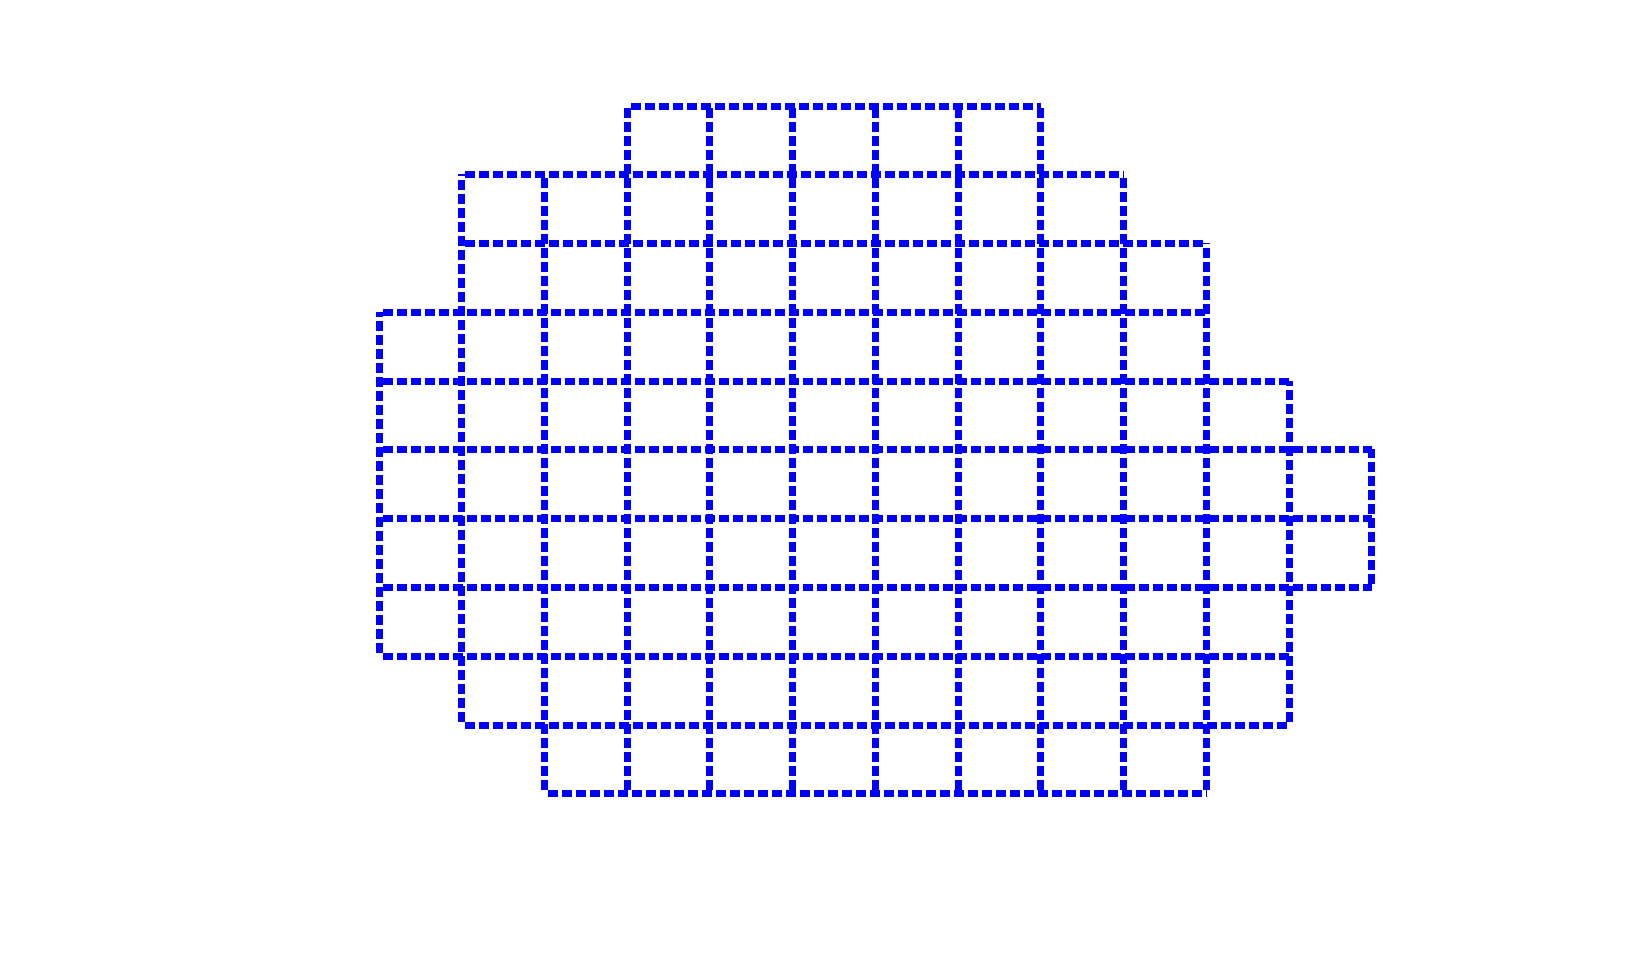
\includegraphics[width=0.3\textwidth]{OG.png}}\hfill
	\subfloat[][]{
	\label{fig:GridGaussian}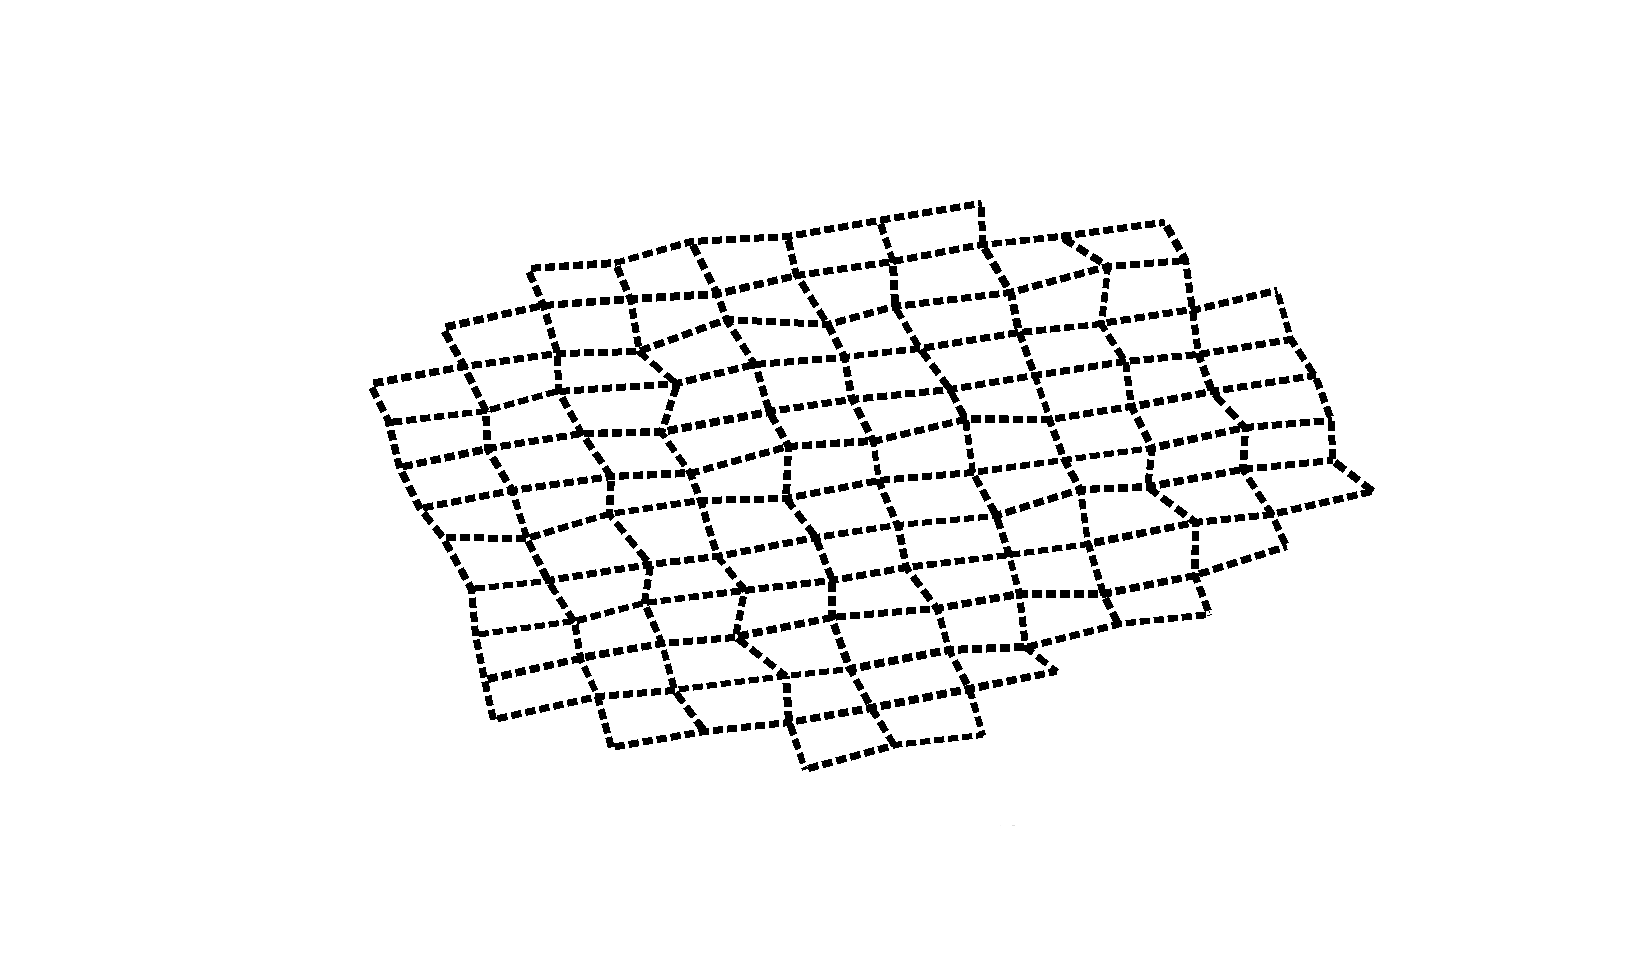
\includegraphics[width=0.3\textwidth]{GG3_80.png}}\hfill
	\subfloat[][]{
	\label{fig:GridBarrel}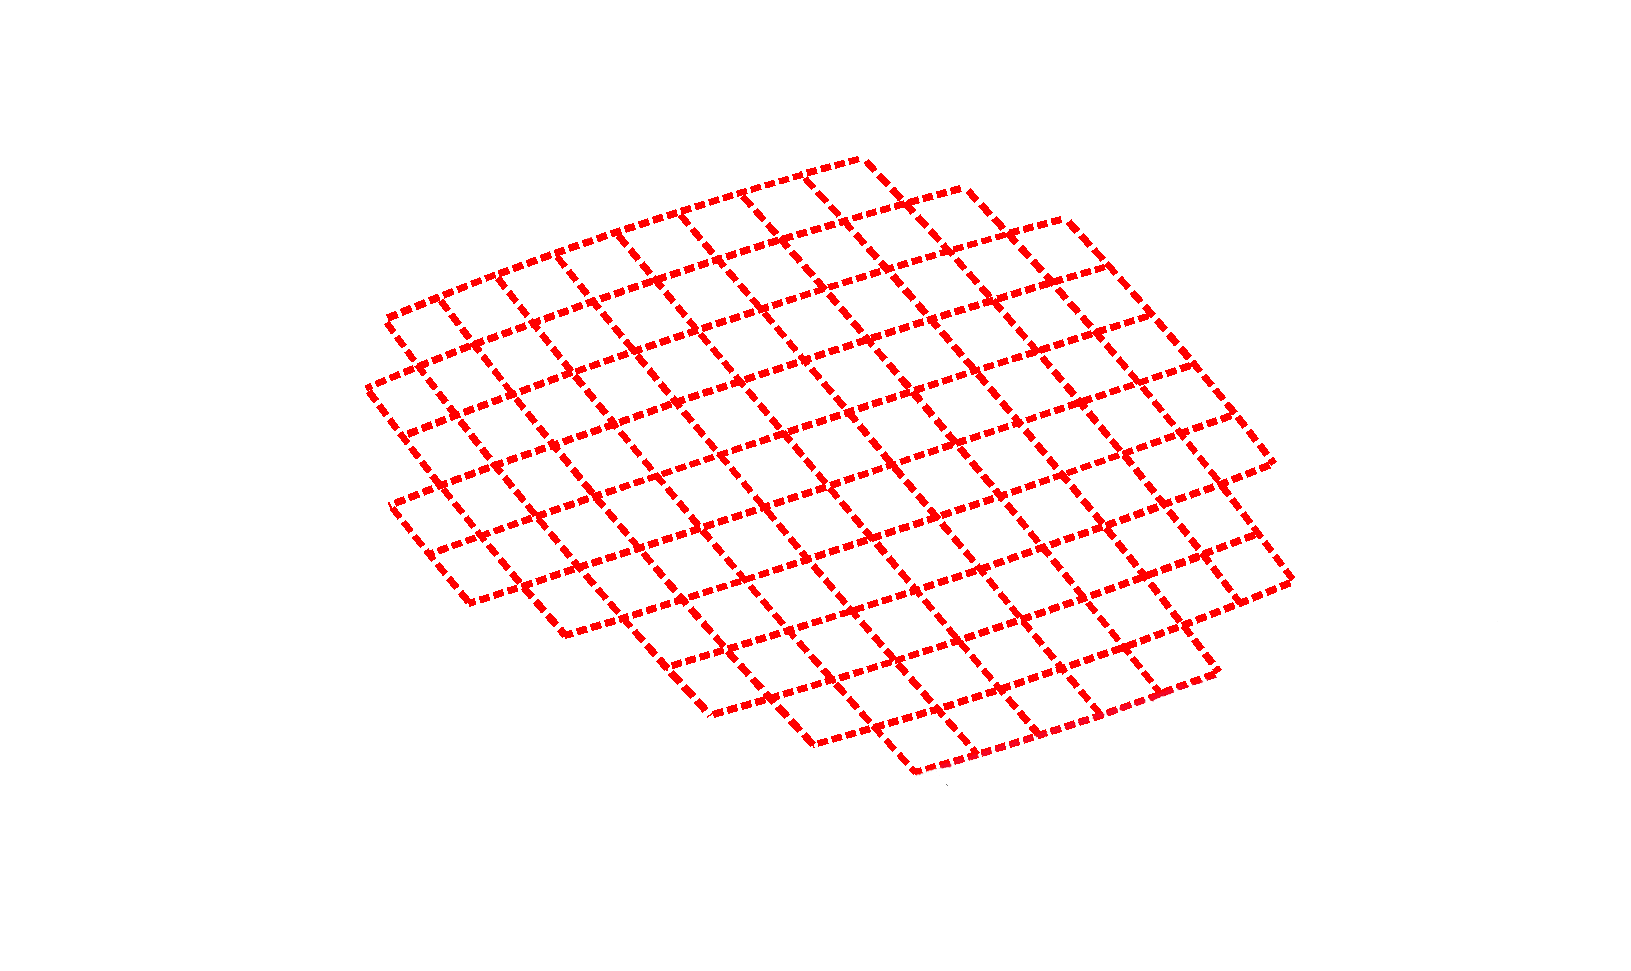
\includegraphics[width=0.3\textwidth]{BG3_145.png}}
	\caption{Data space transformation: \protect\subref{fig:GridOriginal} original synthetic data, \protect\subref{fig:GridGaussian} \acs*{rdgm} deformation, \protect\subref{fig:GridBarrel} \acs*{bd} deformation.}
	\label{fig:DSOS}
\end{figure*}


\section{\uppercase{Material and Methods}}\label{sec:mm}

% Our framework is formulated as a standard classification framework. First the dermoscopy images are represented by a set of elements or features. With reference to our previous studies on melanoma classification \cite{rastgoo2015automatic, rastgoo2015ensemble} the texture and color features with the highest performance are selected. These features include, \Ac{clbp} \cite{guo2010completed}, Gabor filter \cite{Manjunath96-45}, color variance and histogram and hue and opponent angle color histogram \cite{van2006coloring}. The extracted features are explained in the following. The retrieved features are used to train a \Ac{rf} classifier.

\noindent Figure~\ref{fig:schema} illustrates and summarizes the experiment designed to explore the data imbalance problem during the classification of dermoscopic images.
The experimentation is based on the works presented in~\cite{rastgoo2015automatic, rastgoo2015ensemble} and follows a cross-validated classification evaluation framework.
Details of the dataset used for the experiments are given in Sect.\,\ref{sec:dataset}. 
The extracted features correspond to the highest performing subset of features according to the latter mentioned studies and are presented in Sect.\,\ref{sec:feat}.
The balancing strategies are explained in depth in Sect.\,\ref{sec:met} and finally the validation and classification are discussed in Sect.\,\ref{sec:clas-val}.
%We dedicate an entire section (see Sect.\,\ref{sec:met}) to focus on the different balancing strategies.
%The classification is performed using a \ac{rf} classifier with 100 unpruned trees using gini criterion.
%The validation model used is a 10-fold cross-validation in which \SI{80}{\percent} of the data are used for training and \SI{20}{\percent} are used for testing.

\subsection{Dataset}\label{sec:dataset}
In order to allow future comparisons, we choose to work with the only public dermoscopic dataset $PH^{2}$~\cite{barata2013two}.
%The only public dermoscopic dataset $PH^{2}$~\cite{barata2013two} is used in this work, allowing to reuse this comparison in the future after the development of new methods.   
This dataset is acquired at \textit{Dermatology Service of Hospital Pedro Hispano, Matosinhos, Portugal}~\cite{barata2013two} with Tuebinger Mole Analyzer system with a magnification of $20 \times$.
The 8-bits~RGB color dermoscopic images were obtained under the same conditions with a resolution of $\SI{768}{px} \times \SI{560}{px}$. 
This dataset contains 200 dermoscopic images divided into 160 benign and dysplastic and 40 melanoma lesions. 
Moreover, each lesion is segmented and histological diagnosis are provided as ground-truth. 
In this study, we conduct our experiments on a data subset in order to obtain an imbalance ratio of 1:3, which complies with the requirements of the \ac{os} method in the data space.
Thus, the subset is composed of 39 melanoma and 117 benign and dysplastic lesions, randomly selected. 
%Four images are discarded due to artifacts such as hair occlusions. 

\subsection{Feature extraction}\label{sec:feat}

\begin{description}
\item[The color variance and histogram ($C_{1}$)] descriptor contains the mean and variance of the color channels $\{$R, G, B, H, S, V, L, A, B$\}$ and a 42 bins histogram for each channel of the set $\{$R, G, B$\}$. Thus, the final descriptor is made of 144 features.
\item[The opponent color space angle and hue histogram] \textbf{($C_{2}$)} is a robust and rotation invariant feature descriptor derived from the RGB channels~\cite{van2006coloring}, such that:
  \begin{align}\label{Eq:AngO}
    H &= \arctan\left(\frac{\sqrt{3}\left(R-G\right)}{R+G-2B}\right) \ , \nonumber \\
    \theta^{O}_{d} &= \arctan \left( \frac{\sqrt{3}\left(R'_{d}-G'_{d}\right)}{R'_{d}+G'_{d}-2B'_{d}}\right) \ ,
  \end{align}
\noindent where $d$ denotes the spatial coordinates of $(x,y)$ and $R'_{d}$, $G'_{d}$, $B'_{d}$ denote the first order derivatives of RGB channels with respect to the coordinates. 
This color descriptor is built by taking a 42 bins histogram for the opponent angle $\theta^{O}_{d}$ and the hue channel $(H)$, for a final descriptor size of 84 dimensions.
\item[\ac{clbp} ($T_{1}$)] is a completed modeling of \Ac{lbp}, especially designed for texture classification~\cite{guo2010completed}. 
This descriptor encodes the magnitude and sign differences of the central pixel with its neighbors and the grey level of the central points in the local patterns rather than only the sign differences (see Fig\,\ref{fig:CLBPFig}). 
The sign $CLBP_S$, magnitude $CLBP_M$, and central grey level $CLBP_C$ binary pattern are created by encoding the local distance components and the central grey levels to binary patterns.  
The \ac{clbp} are calculated for each pixel in a given image and the final descriptor is defined as their histogram.
The rotation invariant, uniform, and normalized \ac{clbp} features is calculated considering a radius of \SI{24}{px}.

\item[Gabor filter ($T_{2}$)] is a linear filter which is defined as a modulation of a Gaussian kernel with a sinusoidal wave. 
This filter is formulated in Eq.\,\eqref{Eq:Gabor} as two Gaussians with standard deviations of $\sigma_{x}$ and $\sigma_{y}$ that vary along $x$ and $y$ axes and it is modulated by a complex sinusoidal with a wavelength of $\lambda$. 
Here $\theta$ represents the orientation of the Gabor filter, $\psi$ is the phase offset and $s$ is the scale factor. 
The filter bank is created using six different orientations equally spaced in the interval $[0, \pi]$, along 4 scales with a downsizing factor of 2:
\begin{equation}\scriptsize
  \label{Eq:Gabor}
  g(x,y) = \exp{ \left(-\left( \frac{x'^{2}}{2\sigma_{x}^{2}}+\frac{y'^{2}}{2\sigma_{y}^{2}} \right) \right)} \cos\left( 2\pi\frac{x'}{\lambda}+\psi \right) \ , 
\end{equation}
\noindent where
\begin{align*}
  x' &= s\left( x\cos\theta+y\sin\theta\right) \ ,  \\
  y' &= s\left( -x\sin\theta +y\cos\theta\right) \ .
\end{align*}

\end{description}



%%% Local Variables:
%%% mode: latex
%%% TeX-master: ``../../master''
%%% End:
